\section*{\sffamily \Large INTRODUCTION}

Principal component Analysis (PCA) is one of the oldest, yet most widely used methods of unsupervised multivariate analysis. Given a $p$-dimensional random variable $\BX$ with mean vector ${\bf 0}_p$ and covariance matrix $\bfSigma$, the principal component transformation is defined as:
%
\begin{align}
\BX \mapsto \BY = \bfGamma^T \BX
\end{align}
%
where $\bfGamma$ is orthogonal, and $\bfGamma^T \bfSigma \bfGamma = \bfLambda = \diag( \lambda_1, \ldots, \lambda_p); \lambda_1 \geq \ldots \geq \lambda_p \geq 0$. This induces a set of linear transformations on the random vector $\BX$ so that the transformed random variables are uncorrelated with each other, and their variances are ordered from highest to smallest \citep{MardiaKentBibby}. When $\bfSigma$ is positive definite, coefficients for these transformations, i.e. the columns of $\bfGamma$, are given by the eigenvectors of $\bfSigma$ following its spectral decomposition. For a size-$n$ sample from the distribution of $\BX$, say $\bfX = (\bfx_1, \ldots, \bfx_n)^T$, the first principal component gives the linear combination of columns of $\bfX$ which maximizes sample variance:
%
\begin{align}\label{eqn:eqnPCA1}
\bfw_1 &= \argmax_{\| \bfw \| = 1} Var (\bfX \bfw ) = \argmax_{\| \bfw \| = 1} \bfw^T \bfX^T \bfX \bfw
\end{align}
%
and the subsequent principal components are defined as
\begin{align}\label{eqn:eqnPCAk}
\bfw_k &= \argmax_{\| \bfw \| = 1} \bfw^T \bfR_k^T \bfR_k \bfw; \quad \bfR_k = \bfX - \sum_{s=1}^{k-1} \bfX \bfw_s \bfw_s^T \quad \text{for } 1< k \leq p
\end{align}
%
Following a lagrange multiplier approach, the eigenvectors of $\bfX^T \bfX/n$, equivalently the right singular vectors obtained from the singular value decomposition of $\bfX$ provide solutions to (\ref{eqn:eqnPCA1}) and (\ref{eqn:eqnPCAk}).

PCA has seen extensive applications in diverse areas, such as image recognition \citep{AlkandariAljaber15}, finance \citep{AlexanderBook}, climate science \citep{WilksBook} and text mining \citep{BerryCastellanos}, with the inferential goal being reduction of the intrinsic dimensionality of the feature space without losing information. However, because the objective function to be maximized is quadratic, PCA performs poorly in presence of even a small proportion of corrupted observations \citep{XuCaramanisMannor13}. Based on the domain of application, these corruptions can be the result of data heterogeneity \citep{SahaEtal16}, measurement error \citep{Bailey12,HelltonThoresen14}, or may represent structured noise \citep{CandesEtal09}.

Depending on the modelling goals, robust PCA aims to estimate principal components or the underlying low dimensional subspace in presence of corrupted entries in the data matrix. Historically, the instrumental factors behind the evolution of robust PCA methods have been the size and complexity of datasets, availability of computational resources, as well as the nature of corruptions present in the data. Early methods of robust PCA were focused on robustly estimating the population covariance matrix from datasets that are small to moderate in size, and comprised of independent samples: some of which were outliers, i.e. contained corrupted entries. Later on, computational and statistical challenges that surfaced with the advent of high-dimensional datasets having a large number of features were tackled by methods like projection pursuit \citep{LiChen85}, ROBPCA \citep{hubert05} and M-estimation \citep{LocantoreEtal99,Majumdar15}.

The theoretical discussion in this review is composed of two sections, and we discuss the above broad approaches of robust PCA on independent data in further detail in the first of those sections. We devote the other section to Principal Component Pursuit (PCP), which, even though introduced very recently \citep{CandesEtal09}, has motivated a substantial amount of research on the problem of recovering an underlying low-rank structure in the data matrix, rather than the principal components \textit{per se}, in presence of noise. We illustrate the relevance and relative performance of these two types of methods using two real data examples. The first dataset is available in the R package \texttt{rrcov}, and consists of the measurements of 18 image features for 218 buses. In the second example we take the pixel matrices from four image files: the Lenna image, and three images from the extended Yale Face Database B \citep{GeBeKr01,KCLee05} (fifth images for individuals 1, 2 and 28), add noise to some pixels and attempt to recover the original images using robust PCA techniques. The original images and those with added noise are given in Figure~\ref{fig:allimages}. Following this we review the methods of robust PCA in domains that are not multivariate real, for example reproducing kernel hilbert spaces or the space of square-integrable functions, in the section {\it Robust PCA in Other Spaces}. We finish the review with a concluding section that summarizes the paper and identifies focus areas for future research.

\begin{figure}[t]
\centering
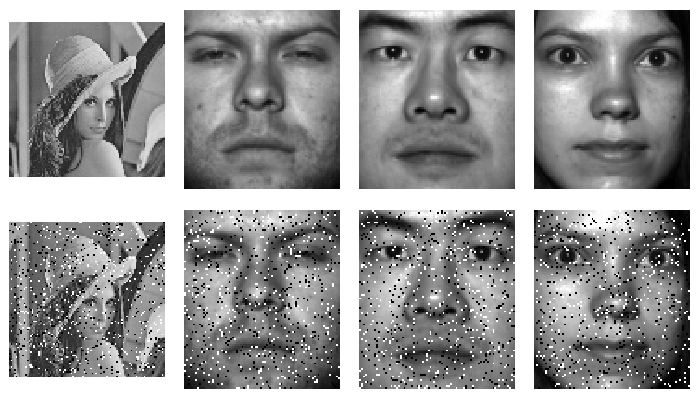
\includegraphics[width=.7\textwidth]{all_images}
\caption{Original and noisy versions of the Lenna image (left) and Yale face images}
\label{fig:allimages}
\end{figure}
